% !TeX root = ../MasterThesis.tex

\documentclass[a4paper,11pt,oneside,titlepage,openany,onecolumn]{scrreprt}

%%%%%%%%%%%%%%%%%%%%%%%%%%%%%%%%%%%%%%%%%%%%%%%%%%%%%%%%%%%%%%%%%%%%%%%%%%%%%%%%%%%%%%

\usepackage{ifthen}
\newboolean{english}
\setboolean{english}{true}


\def\title{Development of a vibrotactile stimulation system for cognitive rehabilitation}
\def\study{Mechatronics \& Smart Technologies}
\def\thesis{Master Thesis}
\def\degree{"Master of Science in Engineering"}
\def\student{Lukas Sieß}
\def\matnr{52010293}
\def\address{6591 Grins, Grins 107H}
\def\reviewerone{Prof. Yeongmi Kim, PhD}


% deutsche Anpassungen
%\usepackage[ansinew]{inputenc}
\usepackage[T1]{fontenc}
\usepackage[ngerman,english]{babel}

% mathematische Symbole
\usepackage{amsmath,amssymb,amsfonts,amstext}

% Listings
\usepackage{listings}
\lstset{numbers=left,numberstyle=\tiny,stepnumber=5,numbersep=5pt}

% erweiterte Zeichenbefehle
\usepackage{pst-all}
\usepackage{hyperref}
\usepackage{glossaries}
\usepackage{booktabs}

% Kopfzeilen frei gestaltbar
\usepackage{fancyhdr}
\lfoot[\fancyplain{}{}]{\fancyplain{}{}}
\rfoot[\fancyplain{}{}]{\fancyplain{}{}}
\cfoot[\fancyplain{}{\footnotesize\thepage}]{\fancyplain{}{\footnotesize\thepage}}
\lhead[\fancyplain{}{\footnotesize\nouppercase\leftmark}]{\fancyplain{}{}}
\chead{}
\rhead[\fancyplain{}{}]{\fancyplain{}{\footnotesize\nouppercase\sc\leftmark}} 

% Farben im Dokument m"oglich
\usepackage{color}

% Schriftart Helvetica
\usepackage{helvet}
\renewcommand{\familydefault}{phv}

% anderdhalbfacher Zeilenabstand
\usepackage{setspace}
\onehalfspacing

% Graphiken einbinden: hier f"ur pdflatex
\usepackage[dvips]{graphicx}

% verbesserte Floating Plazierung
\usepackage{float}

% "Uberpr"ufung des Layouts
\usepackage{layout}

\usepackage{array}

% erweiterte Einstellungen der Bildunterschriften -> 8 Pt
\usepackage[small]{caption}
\captionsetup{belowskip=12pt,aboveskip=4pt}

\usepackage{ifthen}

% H"ohe und Breite des Textk"orpers etwas gr"osser definieren
\usepackage[tmargin=1in,bmargin=1in,lmargin=1.25in,rmargin=1.25in]{geometry}

% Einr"uckung von und Abstand zwischen Abs"atzen
\setlength{\parindent}{0em}
\setlength{\parskip}{1.5ex plus0.5ex minus0.5ex}

% weniger Warnungen wegen "uberf"ullter Boxen
\tolerance = 9999
\sloppy

% Anpassung einiger "Uberschriften 
\renewcommand\figurename{Abbildung}
\renewcommand\tablename{Tabelle}
%\newcommand{\unit}{\mathrm}

% Counter f"ur die Nummerierung
\newcounter{romancount}

% Boolsche Variable f"ur Bachelor-/Masterarbeit oder Bericht
\newboolean{thesis}


\begin{document}
\selectlanguage{english}
\pagenumbering{alph} % use lowercase letters for page numbering
\thispagestyle{empty}
\sffamily

\ThisTileWallPaper{\paperwidth}{\paperheight}{Images/MCIHintergrundKPL.pdf}
%\put(-30,-685){\includegraphics[width=1.15\linewidth]{BG}}

{
	\bfseries

	\vspace*{3.5cm}

	\textcolor{MSBlue}{\sffamily\bfseries\huge\thesis}%

	\vspace*{0.5cm}

	\begin{doublespace} 
		
\textbf{\labtitle{} (\labcode)}

\textbf{\labname}

\textbf{\labdate}	

%Labor \labnum

	%\maketitle
	\vspace*{10cm}

	\textcolor{gray}{\study}

	\def\termname{Semester}
	\textcolor{gray}{\term{ }\termname}

	\def\lecturername{Lector}
	\textcolor{gray}{\lecturername: \lecturer}

	\def\groupname{Group}
	\textcolor{gray}{\groupname: \group}

	\def\authorname{Authors}
	\textcolor{gray}{\authorname: \student}

	\textcolor{gray}{\today}
	\end{doublespace} 
	\newpage
}
\pagenumbering{Roman}  % use uppercase roman numerals for page numbering
\thispagestyle{plain} % format page style for current page
\pdfbookmark[0]{Eidesstattliche Erklärung}{Eidesstattliche Erklärung} % sets a PDF bookmark


\chapter*{Eidesstattliche Erklärung}
\glqq Ich erkläre hiermit an Eides statt, dass ich die vorliegende Arbeit selbstständig angefertigt habe. Die aus fremden Quellen direkt oder indirekt übernommenen Gedanken sind als solche kenntlich gemacht. Die Arbeit wurde bisher weder in gleicher noch in ähnlicher Form einer anderen Prüfungsbehörde vorgelegt und auch noch nicht veröffentlicht.\grqq\\[5\baselineskip]
\vspace{2cm}
\begin{tabularx}{\textwidth}{@{}p{5cm}Xp{5cm}@{}} % @{} eliminates default padding
    \hrulefill & & \hrulefill \\
    Ort, Datum & & Unterschrift
\end{tabularx}
%
\section*{\centering \ifthenelse{\boolean{english}}{Acknowledgement}{Danksagung}}
Text Text Text Text Text Text Text Text Text Text Text Text Text Text Text Text Text Text Text Text Text Text Text Text ...
\newpage

\selectlanguage{ngerman}
\section*{\centering Kurzfassung}
Text Text Text Text Text Text Text Text Text Text Text Text Text Text Text Text Text Text Text Text Text Text Text Text ...

% Bitte 3-5 deutsche Schlagw"orter eingeben, die die Arbeit charakterisieren:
\paragraph*{Schlagw"orter:} Schlagwort 1, Schlagwort 2, Schlagwort 3, Schlagwort 4, Schlagwort 5
\newpage

\selectlanguage{english}
\section*{\centering Abstract}
Text Text Text Text Text Text Text Text Text Text Text Text Text Text Text Text Text Text Text Text Text Text Text Text ...

% Bitte 3-5 englische Keywords eingeben, die die Arbeit charakterisieren:
\paragraph*{Keywords:} Keyword 1, Keyword 2, Keyword 3, Keyword 4, Keyword 5

\newpage

\pdfbookmark[0]{\contentsname}{toc} % sets a PDF bookmark
\tableofcontents
\newcounter{romanpagecount} % create a new counter
\setcounter{romanpagecount}{\value{page}} % capture the current page number
\clearpage
\pagenumbering{arabic} % use Arabic numerals for page numbering
% --> add content of thesis here
\chapter[Introduction]{Introduction}

\section{Motivation and Problem Statement}

%globale Demenzstatistiken (Alzheimer Int., WHO)
\cite{alzint_dementia_statistics}, \cite{who_dementia_factsheet}

%Bedarf an nicht-pharmakologischen Ansätzen
\cite{Zucchella.2018}

%Frühstudien zur 40-Hz-Stimulati (z.B. Gamma-Wellen, Reduktion von Amyloid in Mäusen)
\cite{Mably.2018}, \cite{Iaccarino.2016}, \cite{Martorell.2019}

\section{Objectives of the Thesis}

Erl"autern Sie an dieser Stelle \emph{genau} was ihre Aufgabe ist. Gegebenfalls grenzen Sie auch die Teile aus, welche nicht im Umfang der Arbeit liegen. Dies kann Ihnen gegen Ende ihrer Arbeit bei der Argumentation helfen.

\section{Structure of the Thesis}

Geben Sie in diesem Abschnitt eine grobe Vorausschau auf den Aufbau der Arbeit. Die Arbeit k"onnte empirisch motiviert sein und mit der Auswertung eines Experimentes beginnen oder theoreitsch und somit logischerweise mit einem Theoriekapitel beginnen.


Etst
\chapter[Formatierungen]{Formatierungen von "Uberschriften und Text in Latex}

In Latex brauchen Sie sich um Formatierungen im Prinzip nicht k"ummern. Es ist lediglich notwendig, dass Sie Kapitel, Abschnitte, Unterabschnitte und so weiter als solche deklarieren.

Multiple Leerzeichen        werden von Latex einfach gel"oscht. Haben Sie einen Absatz beendet (nach 3 bis 4 S"atzen), dann lassen Sie durch ein zweimaliges ''Enter'' eine Zeile Abstand. Der Absatz wird je nach globaler Einstellung einger"uckt oder abgesetzt.

Wollen Sie im Text etwas hervorheben, dann verwenden Sie \emph{hervorgehoben}. Die Hervorhebung wird von Latex automatisch dem jeweiligen Textstil angepasst. Sie k"onnen aber auch etwas explizit \textbf{fett}, \textit{kursiv} oder \underline{unterstrichen} setzen, wobei dies mit Vorsicht zu genie"sen ist.

\section[Abschnitt]{Das wäre ein Abschnitt}

Mit etwas Text ...

\subsection[Unterabschnitt]{Bzw. ein Unterabschnitt}

Wie Ihnen vielleicht schon aufgefallen ist, vergr"o"sert \LaTeX nach einem ''.'' den Abstand geb"uhrlich f"ur ein Satzende. Falls dies nicht ben"otigt wird z.B.~hier, sollte dies h"andisch verhindert werden.

\paragraph{Gliederungsebene 3} Die n"achste Gliederungsebene wird nicht mehr nummeriert.

\LaTeX kennt auch Aufz"ahlungen wobei es diese mit
\begin{enumerate}
\item Nummerierung
\item\label{enum-ebene} auf der ersten Ebene
\item oder
\begin{itemize}
\item ohne Nummerierung
\item auf der 2.~Ebene gibt.
\end{itemize}
\end{enumerate}
Es gibt eine ganze Reihe von weiteren Formatierungsm"oglichkeiten. Z.B.~behandelt {\LaTeX} die erste Seite eines Kapitels anders als alle folgenden. Dies f"allt insbesondere bei der Seitenzahl und der Kopfzeile auf.

\chapter{Analysis of the Current VCA-Based System}

\section{Overview of the Current VCA System}
This section provides an overview of the existing Voice Coil Actuator (VCA)-based setup. The System consists of seven main parts. 

\begin{itemize}
    \item Spring frame (Minimizing the loss of vertical motion transmitted to the node)
    \item Magnet Housing (fixed Magnetic field is always formed)
    \item Bobbin Coil (Magnetic field is formed only when current flows)
    \item Node (Transmitting vertical motion directly to the human body as sound and vibration)
    \item Node screw (fixes the node to the bobbin coil)
    \item Rubber frame (Suppresses vibration from the body from being transmitted to the outside world)
    \item Connection PCB (Take the analog signal from the AMP and apply it to the bobbin coil)
\end{itemize}

\section{Dynamic Behavior: Frequency Measurement}

\subsection{Objective}

\subsection{Measurement Setup}


\subsection{Results \& Interpretation}

\begin{figure}[H]
    \centering
    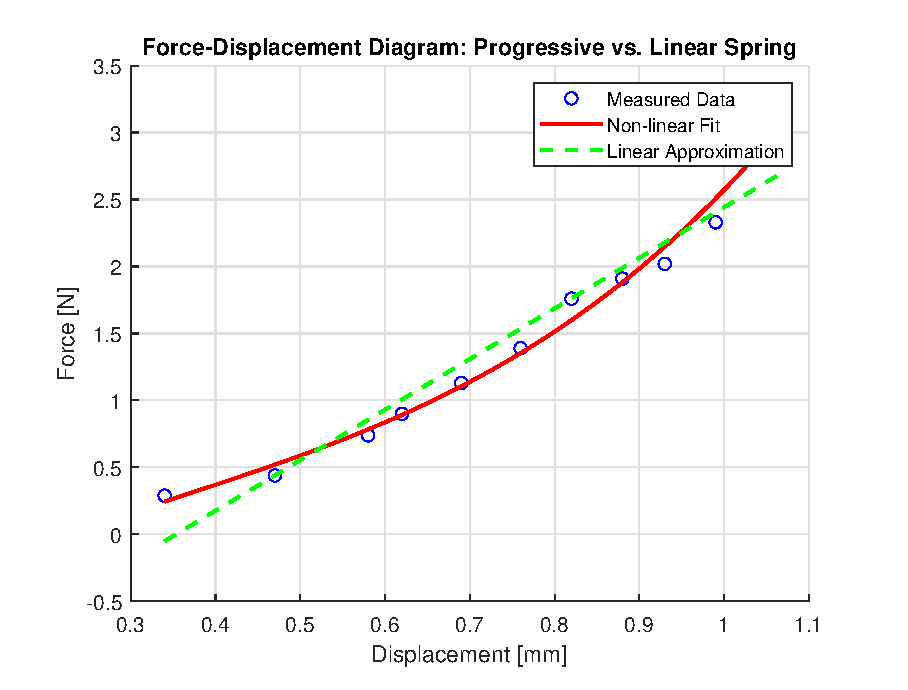
\includegraphics[width=0.62\textwidth]{img/SpringTest.eps}
    \caption[SpringTest]{SpringTest}
    \label{fig:SpringTest}
\end{figure}


\section{Limitations and Identified Challenges}

\chapter[Formatierungen]{Formeln}\label{cha-formeln}

Ein besonderer Vorteil von \LaTeX ist die schnelle und einfache Art Formeln einzugeben. Mit ein wenig "Ubung in der Nomenklatur gehen die komplexesten Ausdr"ucke problemlos von der Hand. Eine einfache Formel sieht folgendermaßen.
\begin{equation}
p_1+\frac{\rho v_1^2}{2}+\rho gh_1=p_2+\frac{\rho v_2^2}{2}+\rho gh_2+\Delta p.
\label{eqn-bernoulli}
\end{equation}
Oft ziehen sich Formeln "uber mehrere Zeilen  
\begin{eqnarray}
\Delta L&=&\int\limits_0^L(1-\cos\varphi)\,dx\approx\int\limits_0^L[1-(1-\varphi^2/2)]\,dx=\frac{1}{2}\int\limits_0^Lw'^2\,dx=\nonumber\\
&=&\frac{B^2\lambda^2}{2}\int\limits_0^L\cos^2\lambda x\,dx=\frac{B^2\lambda^2}{2}\left[\frac{\lambda x-\sin\lambda x\cos\lambda x}{2\lambda}\right]_0^L\approx\frac{B^2\lambda^2L}{4}
\end{eqnarray}
oder sind sehr kompliziert
\begin{eqnarray}
\boldsymbol{\tau}&=&2\mu\mathbf{D}=\mu[\nabla\vec{v}+(\nabla\vec{v})^T]\\
\boldsymbol{\sigma}'&=&\mu'\nabla\cdot\,\vec{v}\,\mathbf{I}=-\frac{2}{3}\mu\,\nabla\cdot(\nabla{v})\,\mathbf{I}.
\end{eqnarray}


\chapter{Evaluation}

\chapter{Zusammenfassung und Ausblick}

\pagenumbering{Roman} % use uppercase roman numerals for page numbering
\setcounter{page}{\value{romanpagecount}} % set page number to the stored value
\stepcounter{page} % increment the page counter
\bibliographystyle{IEEEtran}
\renewcommand\refname{Bibliography}
\bibliography{literatur} % point BibTEX at the .bib files
\addcontentsline{toc}{chapter}{Bibliography}
\clearpage
\listoffigures % generate a list of all the figures
\addcontentsline{toc}{chapter}{\listfigurename}
\clearpage
\listoftables % generate a list of all the tables
\addcontentsline{toc}{chapter}{\listtablename}
\clearpage
\printglossary[type=acronym, title={Abkürzungsverzeichnis}] % input files created by MakeIndex
\appendix
\chapter[Erster Anhang]{Überschrift des ersten Anhangs}\label{app-A}

\lstinputlisting[caption={Test}, label={lst:test_code}]{code/matlab_example.m}


\end{document}